\section{位相雑音抑制手法の概観とフィードフォワード型構成}
\label{sec:methods}

\subsection{既存の量子化雑音抑制手法}

分数分周比PLLの量子化雑音を抑制する手法は，大きく以下の3系統に整理できる．

\begin{enumerate}
  \item \textbf{デジタル-時間変換器（DTC）等によるノイズキャンセル：} MMDの制御列から期待される位相誤差を予測し，DTCで基準経路の時間をずらすことでキャンセルする．ジッタ・電力性能は優れるが，DTCの利得・線形性がプロセス・電圧・温度（PVT）変動の影響を強く受けるため，LMS等のキャリブレーションが必須であり，周波数切替のたびに数十\,$\mu$s〜数\,ms程度の収束時間を要する．
  \item \textbf{ノイズシェーピング周波数を上げる：} DSMの動作周波数（基本構成では基準周波数 $f_\text{REF}$ に一致）を高めることで，量子化雑音をより高域に押しやり，狭いループ帯域でも十分に除去できるようにする．高い基準周波数を得るための逓倍回路が別途必要になる．
  \item \textbf{等価FIRフィルタによる追加フィルタリング：} 主ループの帯域特性は変えずに，遅延の異なる複数の帰還信号を重み付き加算することで量子化雑音だけを追加的に整形する．経路間のゲイン・線形性のマッチングや遅延線の消費電力が課題となる．
\end{enumerate}

第\ref{sec:pll-basics}節で述べた，帰還を高調波ミキサによる「引き算」に置き換える手法（HMベース帰還）は，これら3系統とは異なる「新しいつまみ」として近年注目されており，他の手法と組み合わせることも可能である．

\subsection{HMベースPLLにおける補助PLLのオーバーヘッド}

HMベース帰還を用いるPLL（Dual-Feedback PLLなど）は，量子化雑音の増幅を回避できる一方，HM用の局部発振信号を生成する補助PLLが新たに必要になる．この補助PLLに含まれるVCOの位相雑音は，主ループの外側から加わる雑音源として出力に漏れ込むため，量子化雑音を抑えた代わりに補助VCOの雑音・消費電力のオーバーヘッドが新たな課題として生じる．

\subsection{最近提案されたフィードフォワード（FF）型構成}

この補助VCOのオーバーヘッドを軽減する手法として，Zhangら\cite{zhang_ffnc_2025}は電圧領域のフィードフォワード雑音キャンセル（Feed-Forward Noise Cancellation, FFNC）を提案している．この手法は，補助PLL側のPD出力（＝補助VCOの位相雑音の情報を含む信号）を，そのまま主ループのPD出力に加算するというものである．時間領域で位相を補正する高速遅延線（VCDL）を必要とせず，カスケード接続された2段目のPD出力の時点で信号がすでに低周波の電圧領域に落ちていることを利用して，低速なアンプと抵抗加算のみでキャンセルを実現している点が特徴である．65\,nm CMOSで試作した結果，106\,fs$_\mathrm{rms}$のジッタと$-63$\,dBcの最悪フラクショナルスパーを達成し，キャリブレーション不要という利点を保ったまま最先端級の性能を実証している．

\begin{figure}[H]
  \centering
  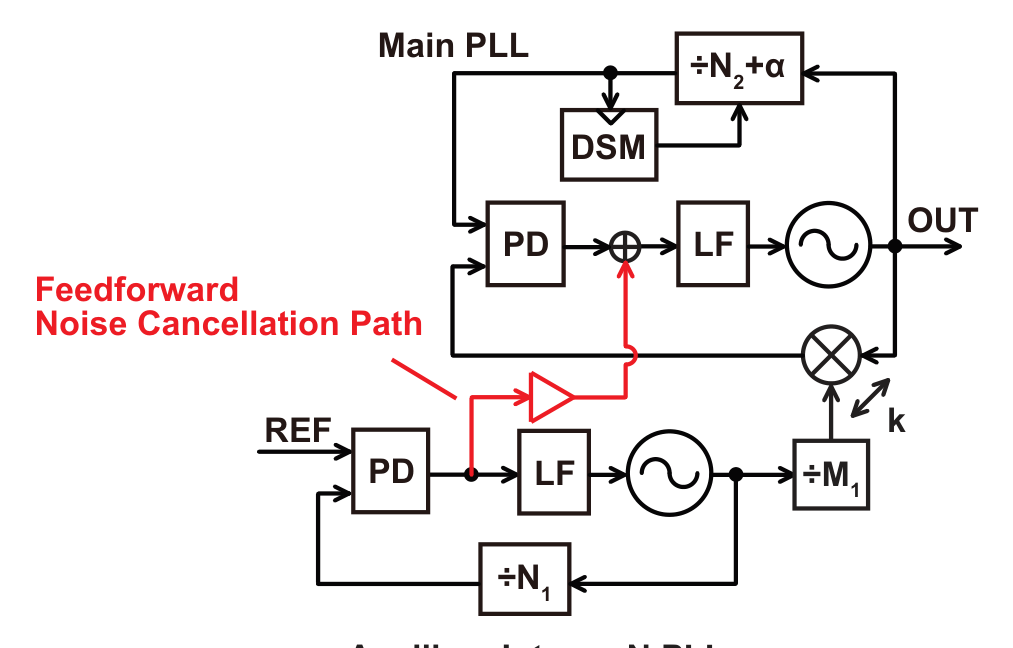
\includegraphics[keepaspectratio,width=0.85\columnwidth]{fig/fig_6_5.png}
  \caption{フィードフォワード雑音キャンセルの基本概念．補助PLLのPD出力を，電圧のまま主ループのPD出力に足し込むことで，高速な遅延線を使わずに補助VCOの雑音成分を打ち消す（\cite{zhang_ffnc_2025}, \cite{osada_thesis}第6章）．}
  \label{fig:ff-concept}
\end{figure}
